\section{EXPERIMENTS}
\label{sec:experiments}



\begin{figure*}[t]
\centering%%% not \center
% \subfigure[Variation with $k$ for $n=10$, $b=5$, made monotonic]{%
% \label{fig:exp-b}%
% 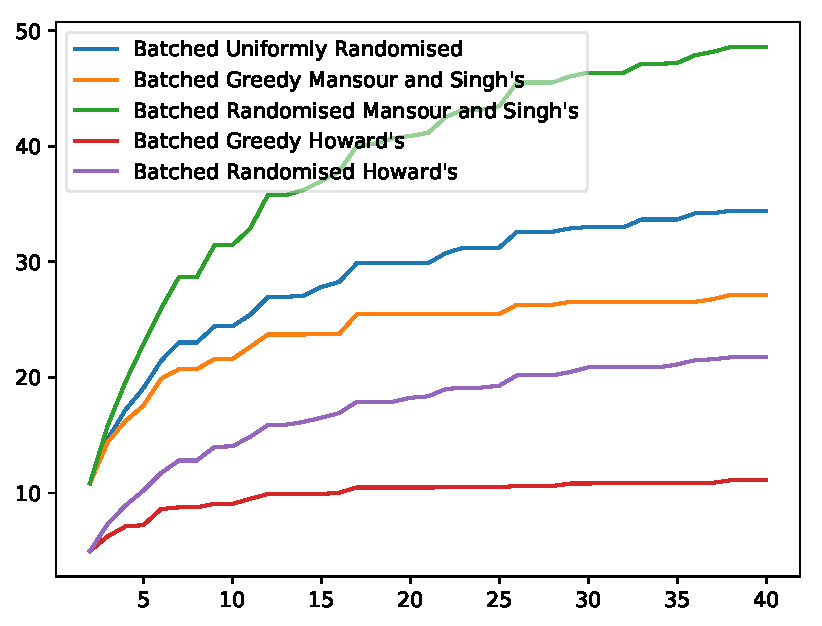
\includegraphics[width=0.5\textwidth]{figs/variation-with-k-monotonized}%
% }
\subfigure[]{%
\label{fig:exp-k}%
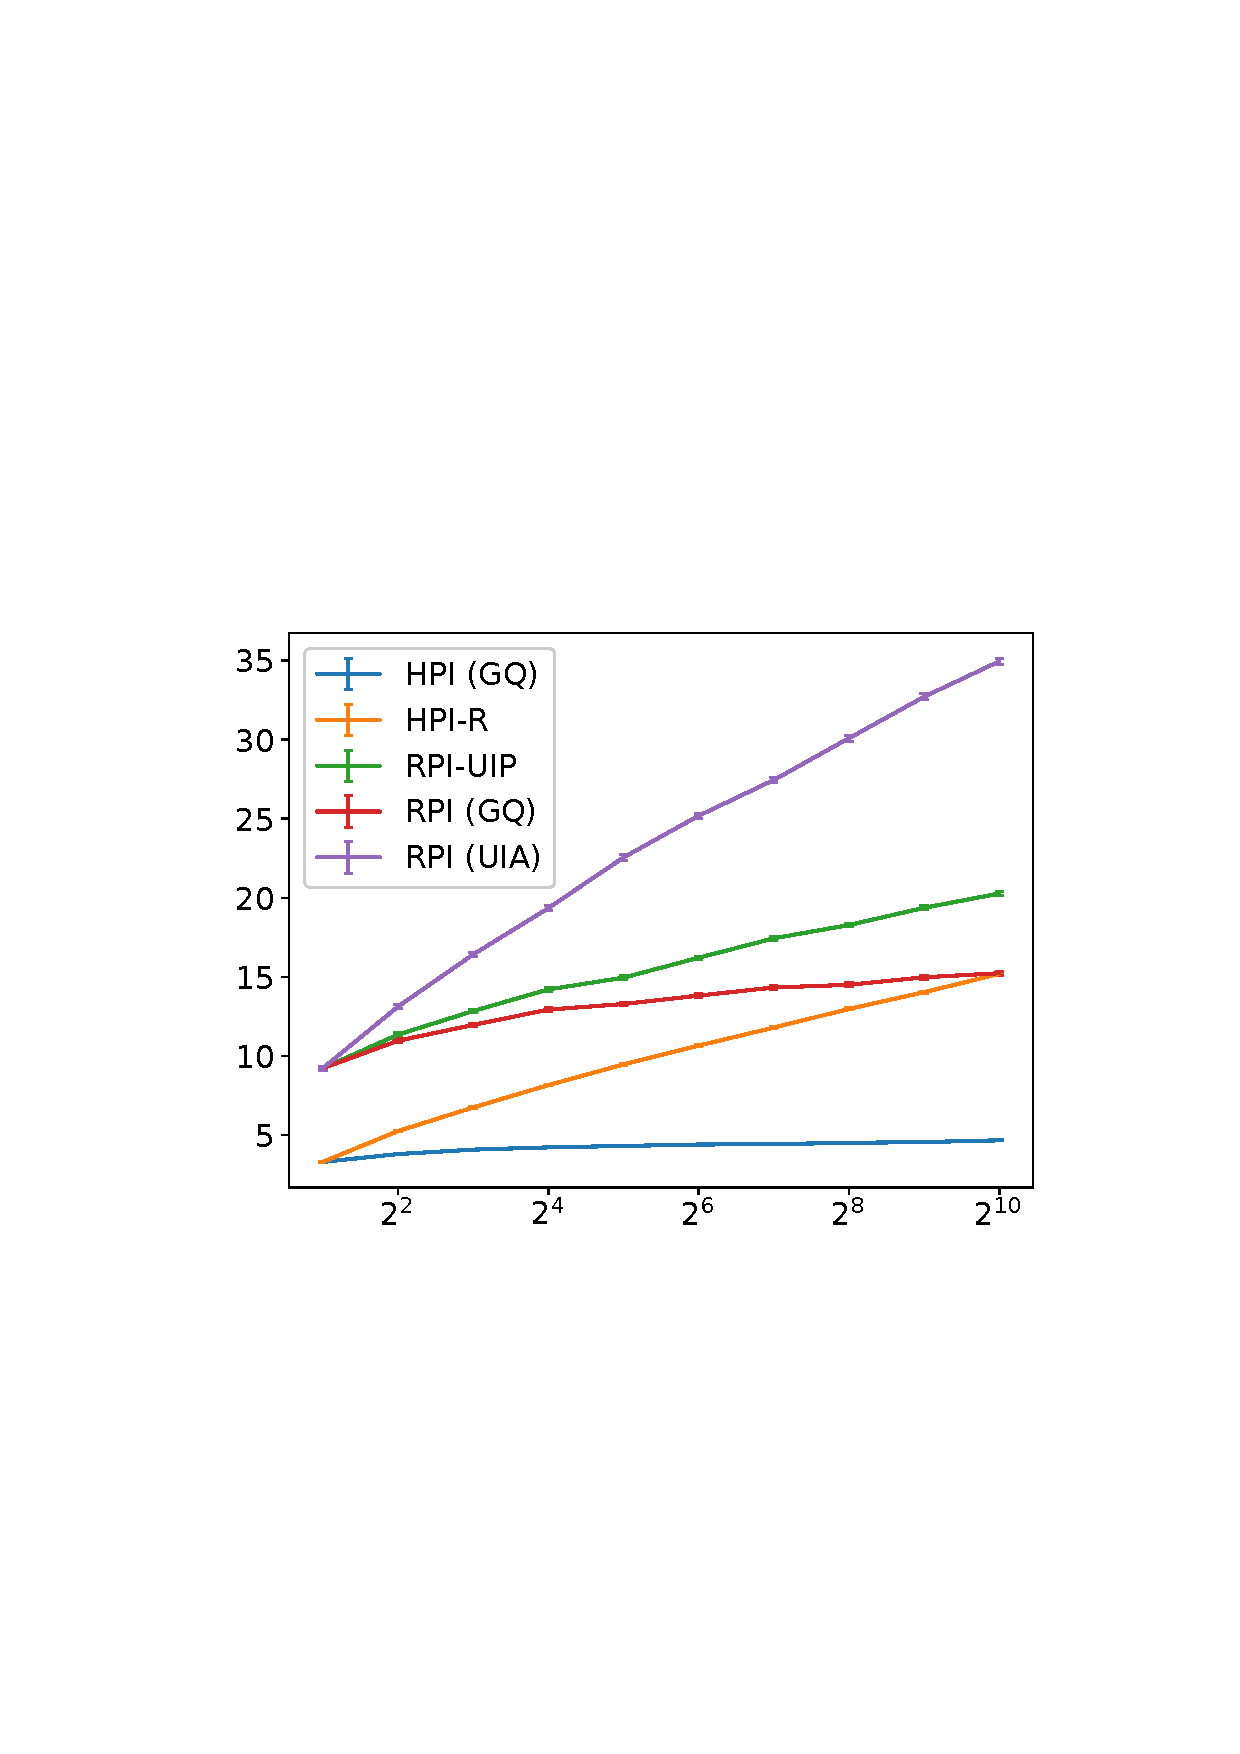
\includegraphics[width=0.25\textwidth]{figs/variation-with-k-logscale}%
}%
\hspace{0.5cm}
\subfigure[]{%
\label{fig:exp-b}%
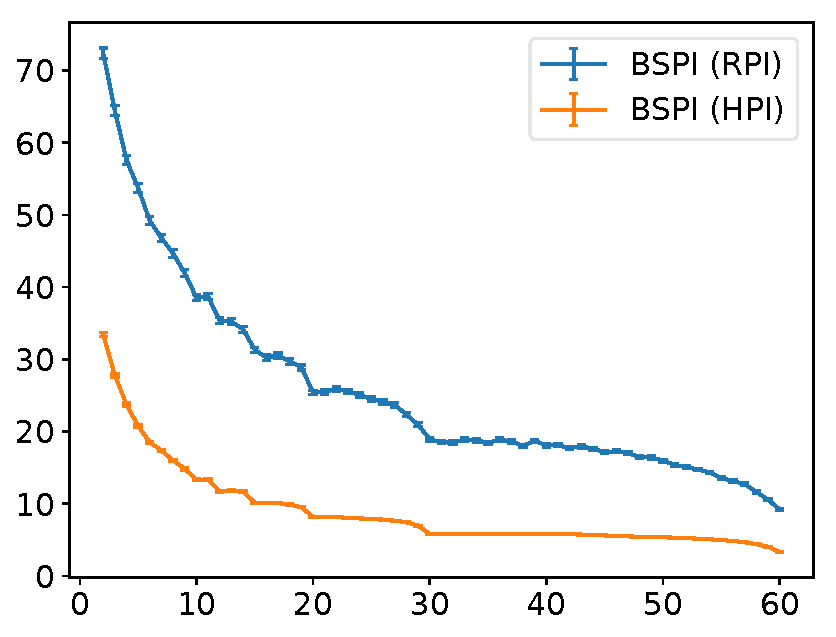
\includegraphics[width=0.25\textwidth]{figs/variation-with-b}%
}%
% \subfigure[Variation with $n$ for $k=6$, $b=5$]{%
% \label{fig:exp-d}%
% 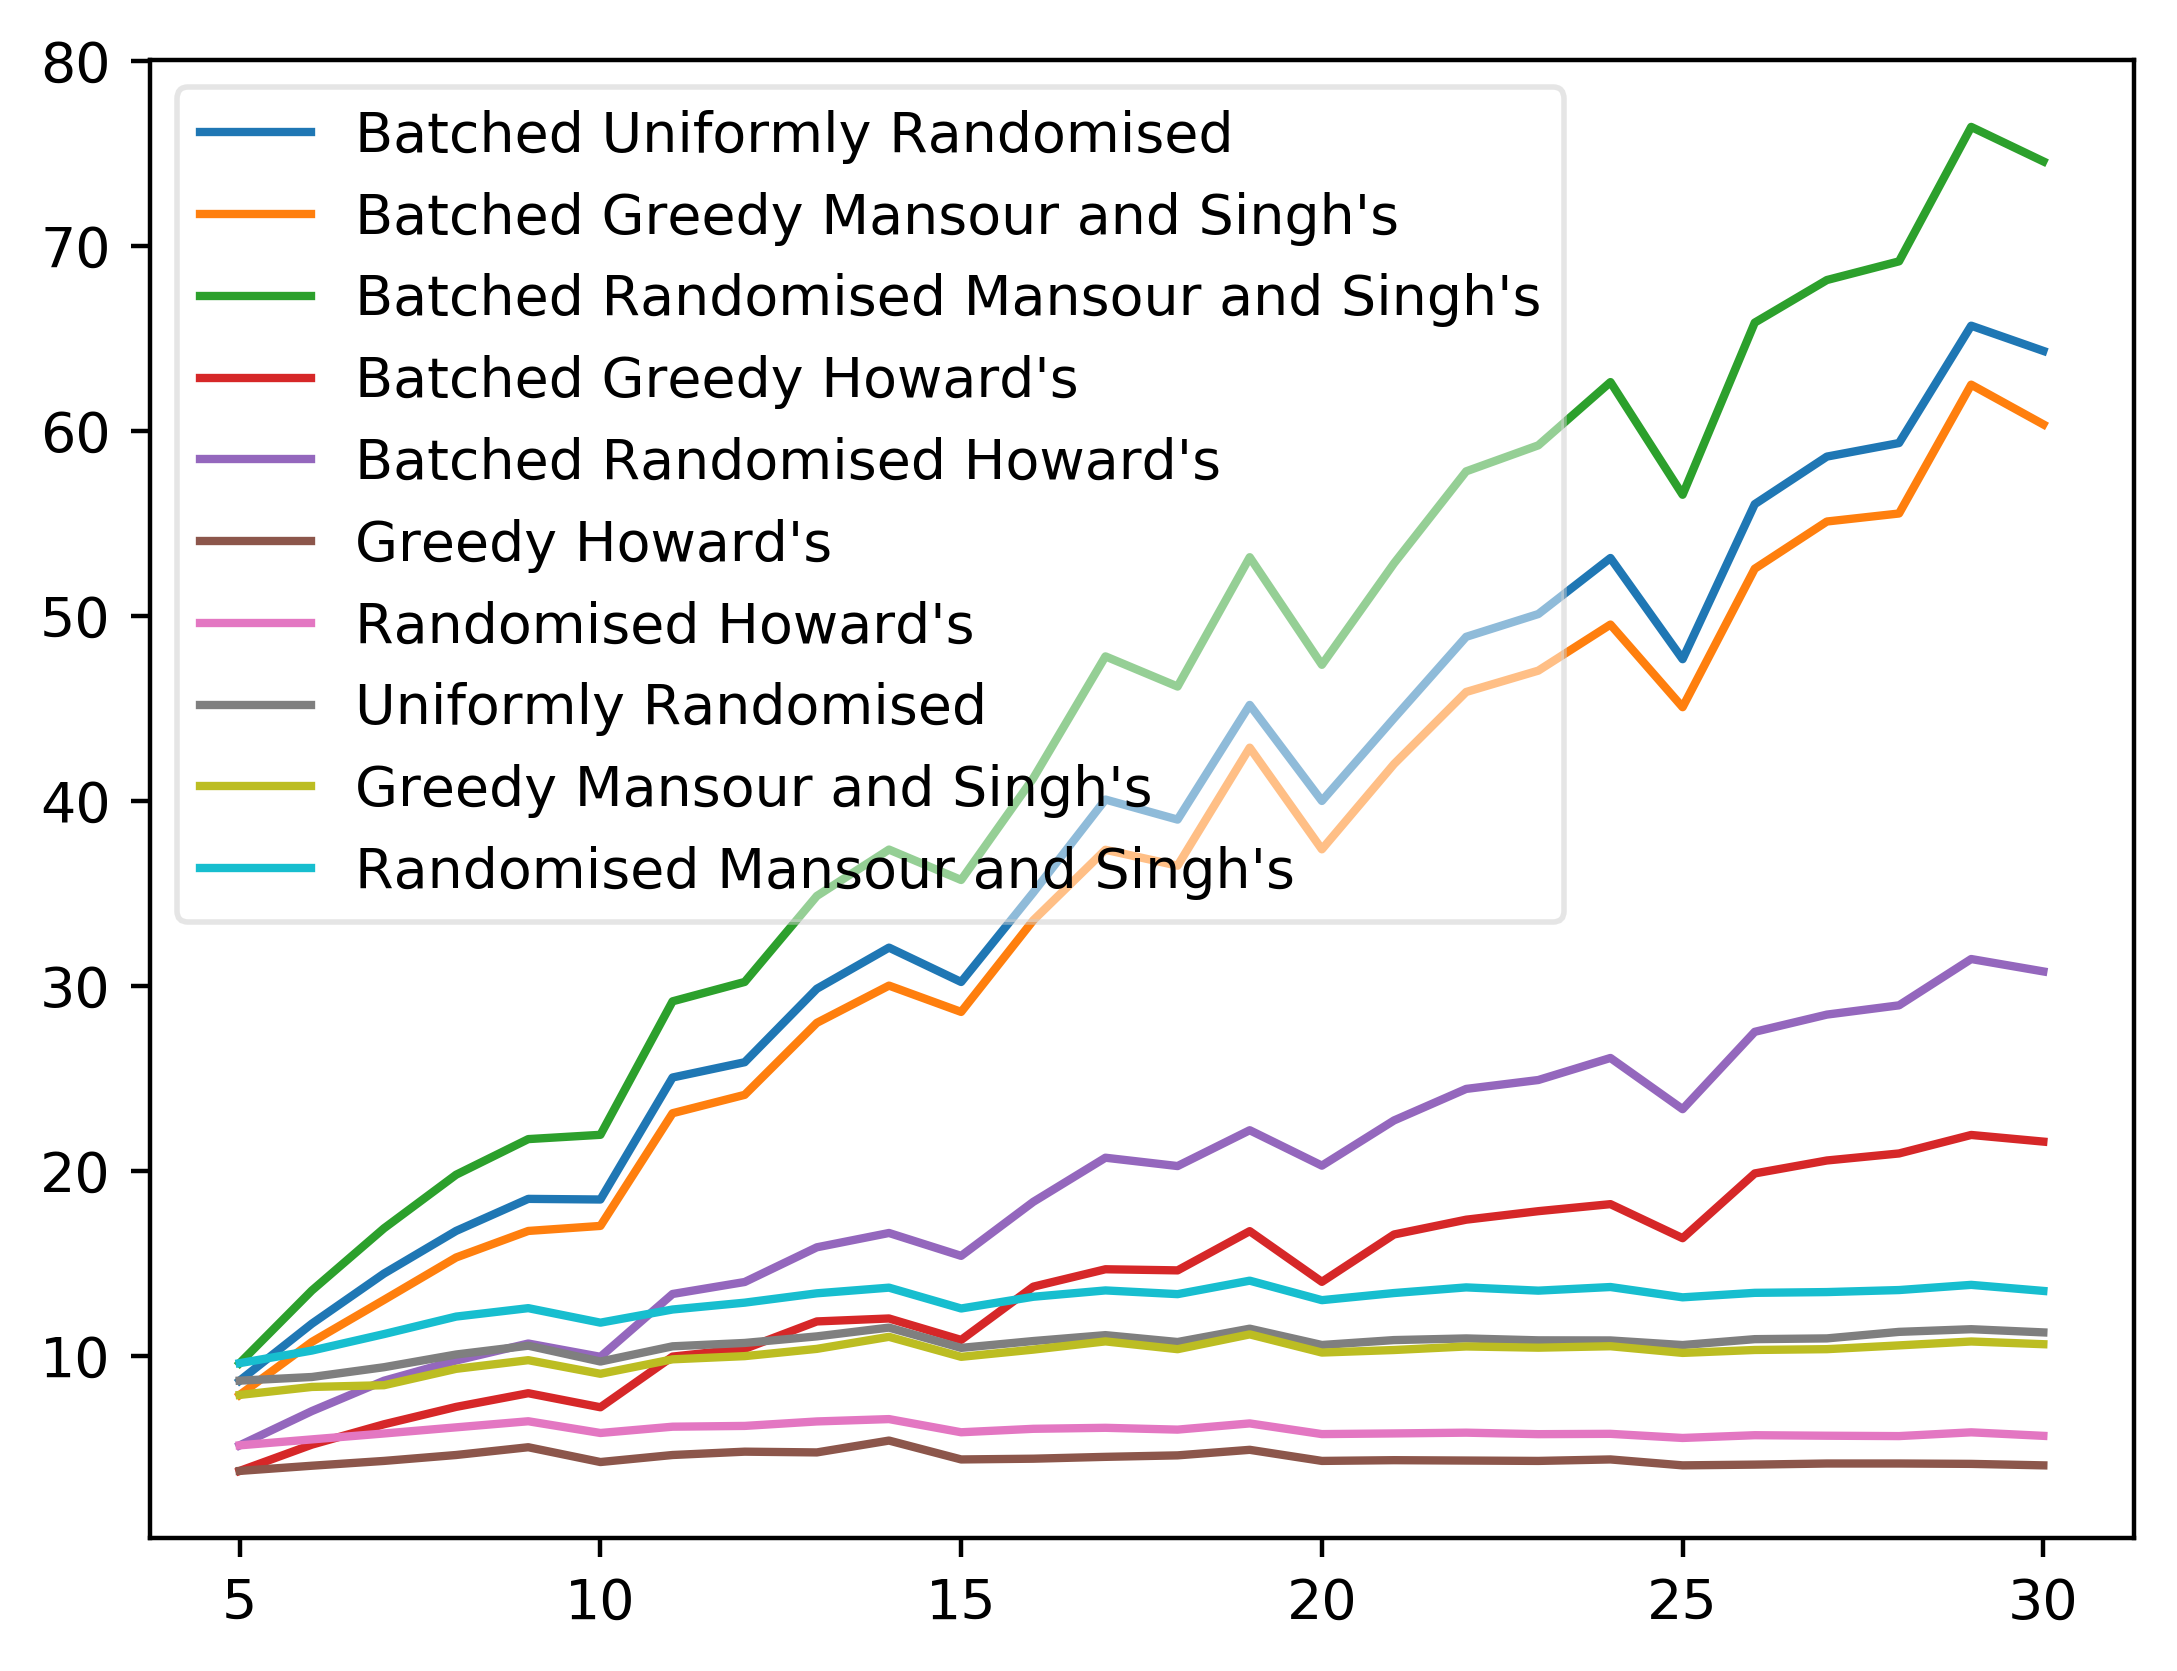
\includegraphics[width=0.5\textwidth]{figs/variation-with-n}%
% }%
\caption{Expected iterations (y axis) against number of actions $k$ in (a) and against batch size $b$ in (b). Each point is an average from 500 independent runs; error bars show one standard error. PI variants HPI (GQ) and RPI (UIA) are described in Section~\ref{sec:experiments}.}
\label{fig:experiments}
\end{figure*}
Interestingly, although the paper by Mansour and Singh~\shortcite{Mansour+Singh:1999} is nearly twenty years old, we are not aware of an experimental comparison between RPI and HPI  published in the literature. We present an experimental comparison of these methods and the variants discussed in this paper, summarising our results in Figure~\ref{fig:experiments}. 

Unlike our theoretical bounds, which are \textit{maximised} over MDPs, each graph plots an \textit{average} over $500$ randomly generated MDPs. In the same manner as  Kalyanakrishnan \textit{et al.}~\shortcite{Kalyanakrishnan+MG-bspi:2016}, we generate an $n$-state, $k$-action MDP by uniformly sampling $n / 5$ possible successors for each of the $nk$ state-action pairs. For each $(s,a,s^{\prime})$ triple thus obtained, the reward $R(s,a,s^{\prime})$ is drawn from a standard normal distribution; $P(s,a,s^{\prime})$ is drawn uniformly from $[0,1]$ and thereafter normalised. The remaining rewards and probabilities are set to $0$. We take $n = 60$ and $\gamma =  0.99$. The starting policy for PI on each MDP is picked uniformly at random.


Figure~\ref{fig:exp-k} compares variants of HPI and RPI as $k$ is varied. Our first observation is that running HPI with greedy action selection based on the $Q$-function (GQ) is by far the most efficient variant.  HPI-R comes second for small values of $k$. Among RPI variants, too, GQ switching performs the best. Note that GQ-switching is only applicable to MDPs, whereas the other variants apply more generally to AUSOs. RPI-UIP consistently takes fewer iterations than than RPI (UIA), a variant of RPI~\cite{Mansour+Singh:1999} in which improving actions are picked uniformly at random from chosen improvable states, which are themselves first selected uniformly at random.

Figure~\ref{fig:exp-b} assesses the effect of using RPI within the batches of BSPI, comparing it with the canonical approach of using HPI~\cite{Kalyanakrishnan+MG-bspi:2016}. This experiment uses $k = 2$. For every fixed batch size $b$, we find that the HPI-based variant performs better in aggregate. Both variants show the same trend: a fairly consistent drop in the number of iterations as $b$ is increased. If it can be proven that a larger batch size implies a tighter upper bound for RPI-based BSPI, it would follow that our bound of $1.6001^{n}$, obtained by analysing $4$-AUSOs, also applies to RPI itself (as it is equivalent to BSPI with a batch size of $n$). Such a result would improve the current bound of $O(1.7172^{n})$ iterations for RPI substantially.

\begin{comment}

~\cite{Mansour+Singh:1999}

\end{comment}

% \begin{figure*}[t!]
% \centering   %%% not \center
% \subfigure[]{
% 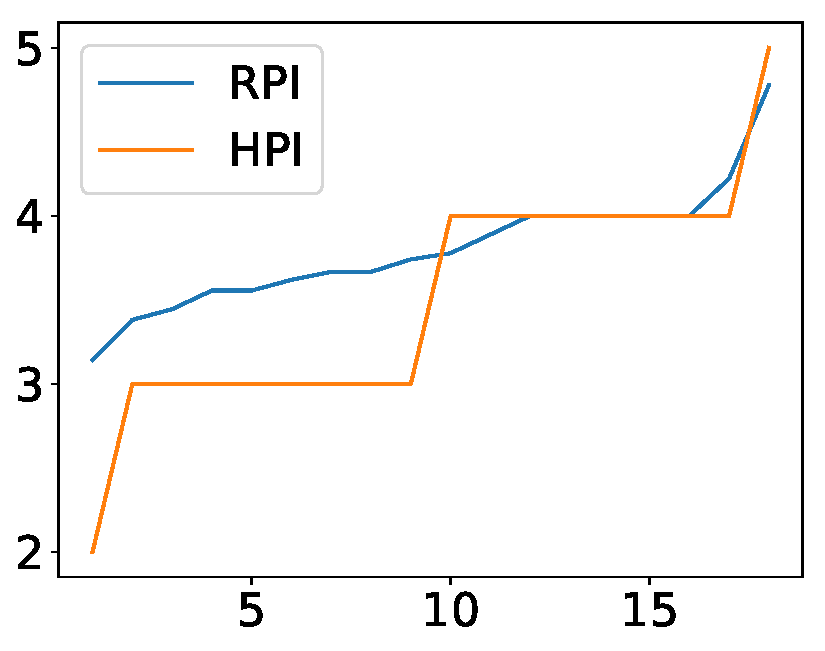
\includegraphics[width=0.245\textwidth]{figs/3-auso}
% }
% \subfigure[]{
% 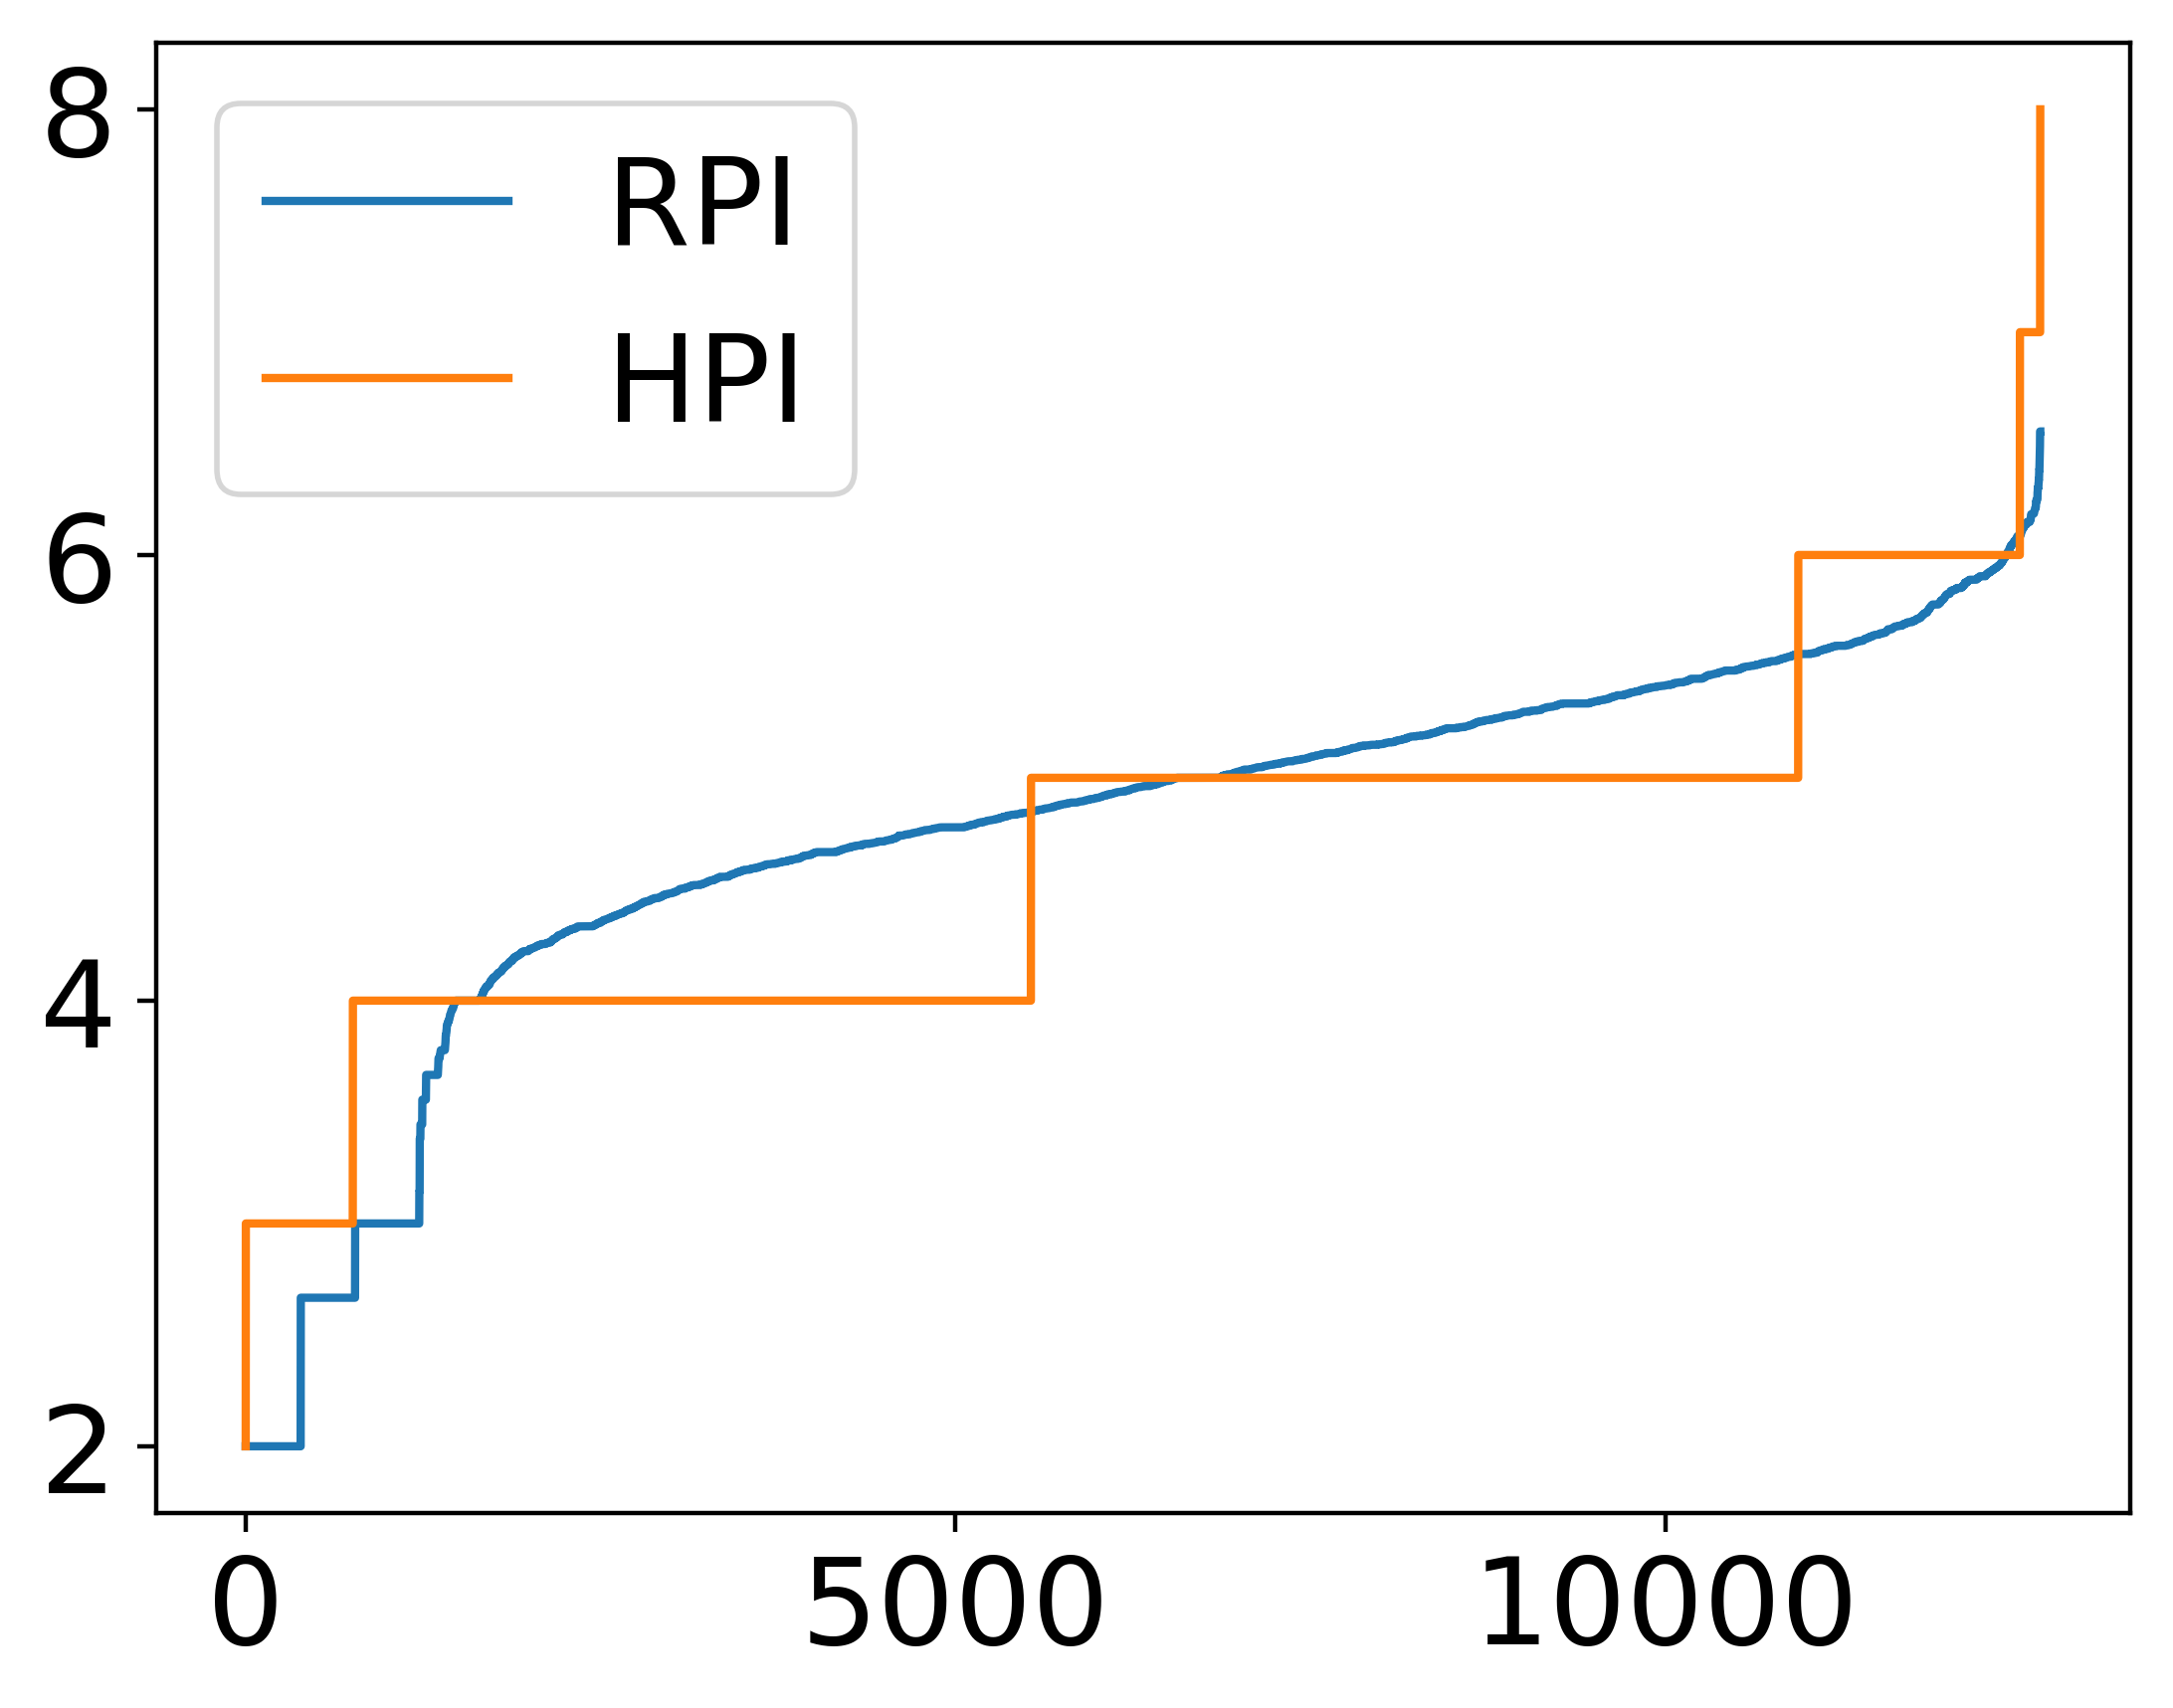
\includegraphics[width=0.245\textwidth]{figs/4-auso}
% }
% \subfigure[]{
% 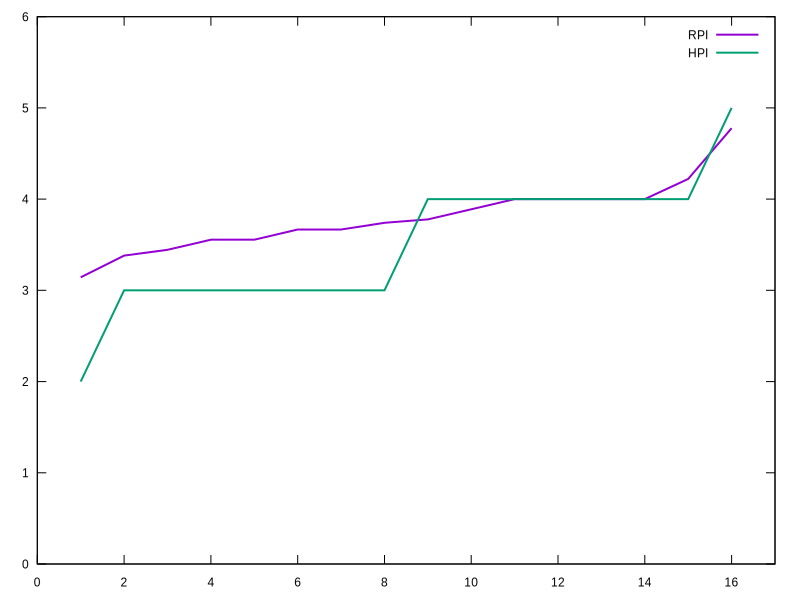
\includegraphics[width=0.245\textwidth]{figs/3-hk-auso}
% }
% \subfigure[]{
% 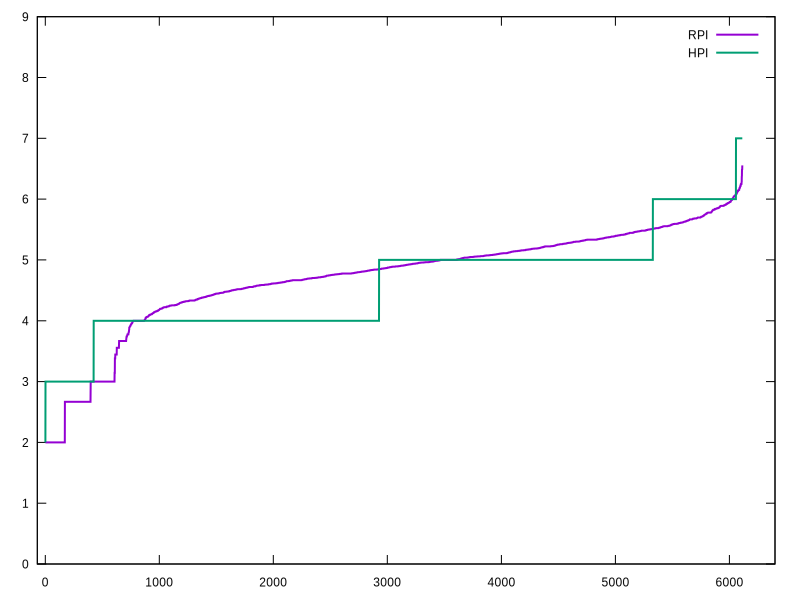
\includegraphics[width=0.245\textwidth]{figs/4-hk-auso}
% }
% \caption{Shivaram will fill out.}
% \label{fig:auso-data}
% \end{figure*}
% 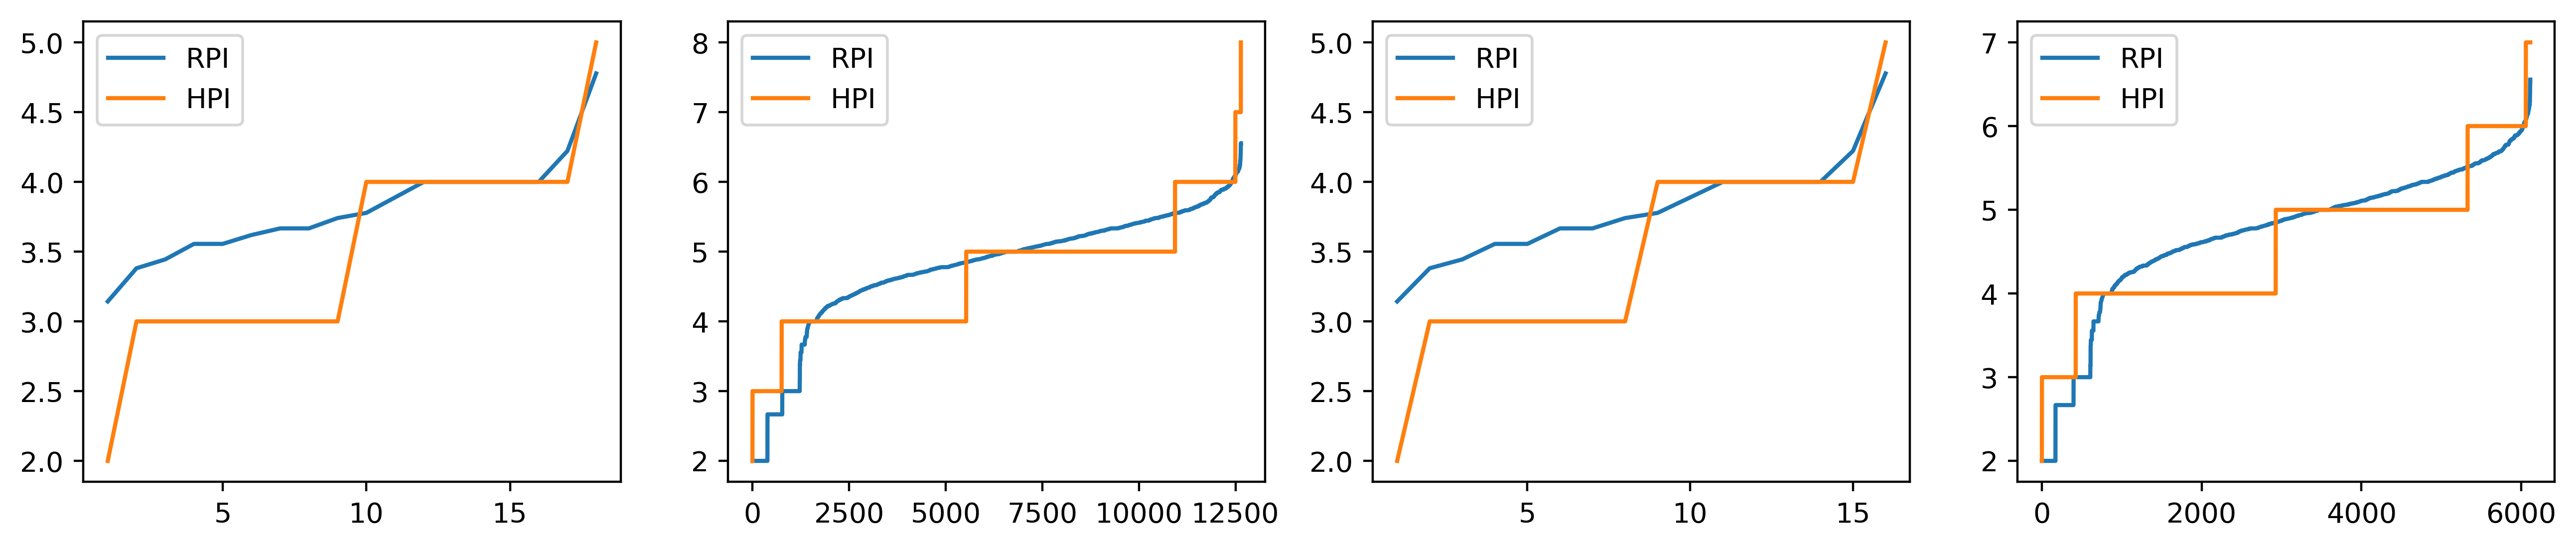
\includegraphics[width=\textwidth]{figs/auso_data.png}


